\section{Architecture}
\label{sec:arch}

\begin{figure*}[t]
  \centering
  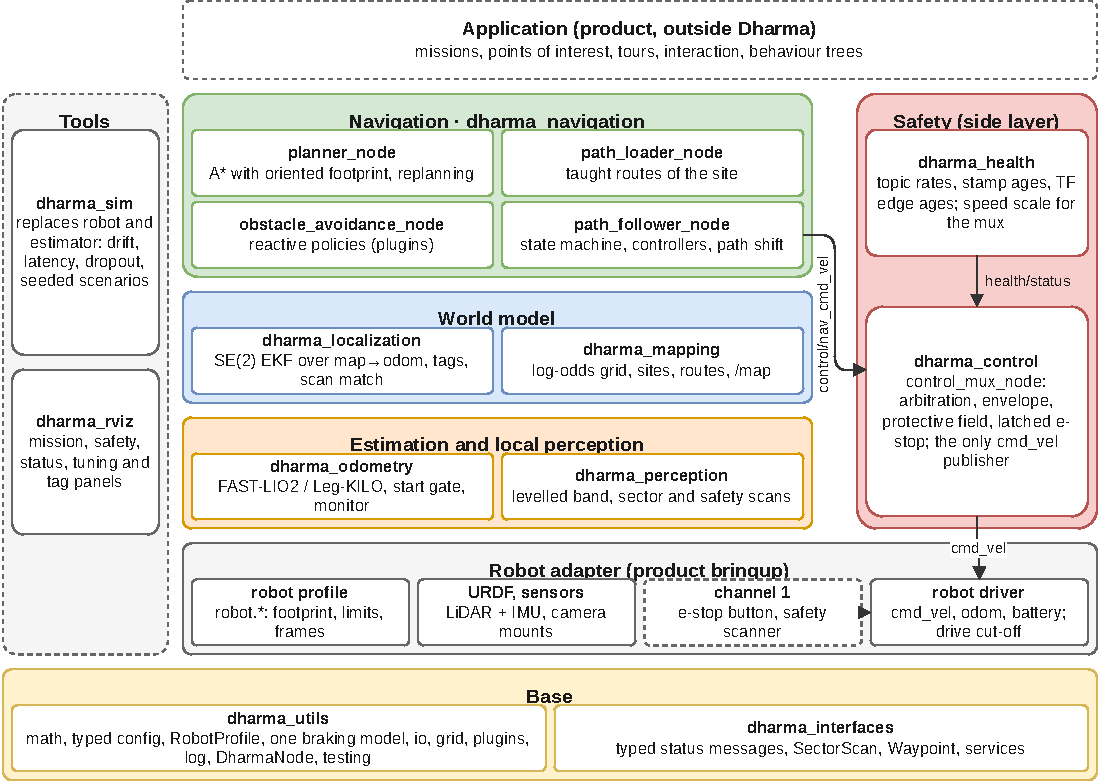
\includegraphics[width=0.92\textwidth]{layers}
  \caption{Layers of Dharma. Every layer depends only on the layers below it and on the base
    (\pkg{dharma\_utils}, \pkg{dharma\_interfaces}); the safety layer sits beside them and is
    the last gate before the robot driver. Colours: estimation orange, world model blue,
    navigation green, safety red, base yellow, hardware grey.}
  \label{fig:layers}
\end{figure*}

\textbf{Layers.} Fig.~\ref{fig:layers} shows the stack. The robot adapter belongs to the product
(driver, URDF, sensor mounts and the robot profile). Estimation and local perception turn raw
LiDAR, IMU and camera data into odometry and obstacle sectors around the robot; the world model
holds the map, the sites and the correction from odometry to the map; navigation plans and
follows paths and docks onto a fiducial-marked charger. Safety is a separate package beside all
layers: one control multiplexer is the only publisher of the robot's velocity command, and a
health monitor turns degraded sensing into a requested speed scale. Each repository depends only on the two base packages, and the
product bringup composes the package launch files.

\textbf{One robot profile.} Every node reads the same \param{robot.*} parameters, parsed into
an immutable \texttt{RobotProfile}: kinematics (omnidirectional or differential), base height
above the floor, a rectangular footprint (front, rear, half width), motion limits (speeds,
acceleration, braking deceleration, yaw deceleration, reaction time) and frame names. Derived
quantities are computed, not copied: the inscribed radius $r_{\mathrm{in}} = \min(f, b, w)$,
the circumscribed radius $r_{\mathrm{c}} = \sqrt{\max(f,b)^2 + w^2}$, the self filter of
perception and mapping, the height band above the floor, the lateral speed limit
($v_y = 0$ for differential robots). For the default profile ($f = b = 0.40$~m, $w = 0.28$~m)
$r_{\mathrm{in}} = 0.28$~m and $r_{\mathrm{c}} = 0.49$~m; the original planner used
$0.35$~m, so a path it accepted could swing a corner of the body about 14~cm into a wall while
turning. The profile validates cross-field consistency (no lateral speed for a differential
robot, distinct frames).

\textbf{Typed configuration.} Each node declares its parameters as frozen dataclasses whose
fields carry a default, unit, range, choices, description and a \emph{live} flag. The node
helper turns them into ROS parameter descriptors, validates every value at start and on every
\texttt{ros2 param set} (rejecting it with a reason), reports unknown parameters (typos) and
makes safety values read-only at runtime. A node that receives an invalid safety parameter
refuses to start instead of running with a default.

\textbf{Plugins and typed interfaces.} Controllers and avoidance policies implement abstract
base classes and register in a named registry that is also open to Python entry points, so a
product adds an implementation without forking. All status topics are typed messages with enum
constants (odometry, localization, mapping, site, planner, navigation, control, health) instead
of strings; safety-relevant actions are separate trigger services so that a default request
can never release or stop something.

\begin{figure}[t]
  \centering
  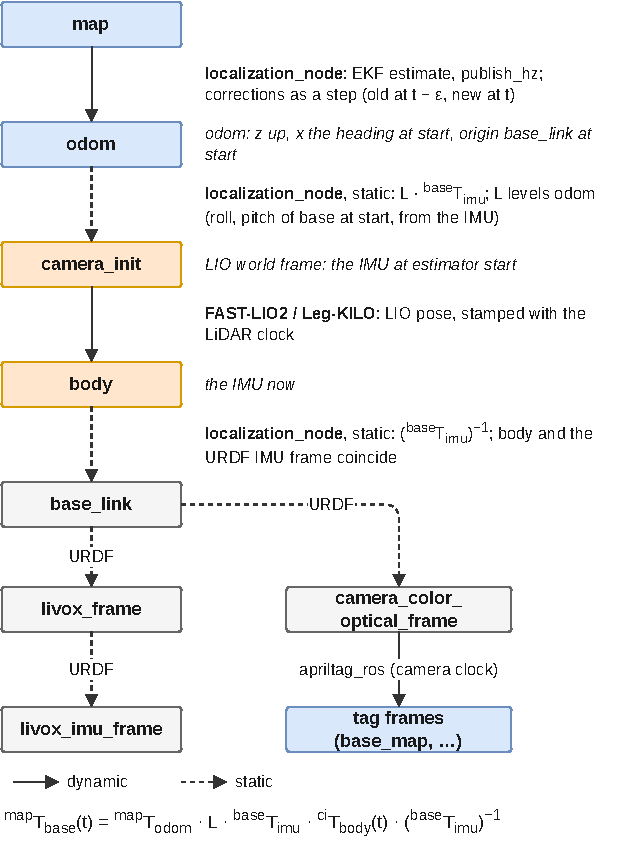
\includegraphics[width=\columnwidth]{tf_tree}
  \caption{TF tree. The LiDAR-inertial odometry publishes \frm{camera\_init}$\to$\frm{body};
    localization adds the static bridge (with the level rotation $L$) and the map correction.}
  \label{fig:tf}
\end{figure}

\textbf{Frames.} The tree follows REP-105 (Fig.~\ref{fig:tf}):
\frm{map}$\to$\frm{odom}$\to$\frm{camera\_init}$\to$\frm{body}$\to$\frm{base\_link}, where
\frm{camera\_init} is the IMU frame at estimator start and \frm{body} the IMU now. The pose of
the robot in the map is
\begin{equation}
  \T{map}{base}(t) = \T{map}{odom}\; L\, \T{base}{imu}\; \T{ci}{body}(t)\;
  \T{imu}{base},
  \label{eq:chain}
\end{equation}
with the static mounting $\T{base}{imu}$ from the URDF, $\T{imu}{base}$ its inverse and the
level rotation $L$ of Sec.~\ref{sec:bridge}. Frame names come from the profile; nothing is hard-coded.
